% This is part of the EPRV project 
% Copyright 2022 the authors

% on GitHub at https://github.com/davidwhogg/EPRV2
% on Overleaf at https://www.overleaf.com/project/61d48c6072be8609b278bda7

% to-do list
% ----------
% - Look for all instances of HOGG, BEDELL, and CITE.
% - Resolve all Overleaf (tm) comments.
% - Make an acronym command and fix CLRB, RV, and all other acronyms.
% - Be sure to discuss SNR in a continuum resolution element, as well as in a pixel.
%.- Make sure that, for any assumption that is explicitly tested, the forthcoming test is mentioned when the assumption is introduced.
% - Are we consistent in our use of Doppler shift, radial velocity, and redshift and so on? Fix figure captions so the figures are clearly in RV. Edit radial Doppler assumption section to say that the terms are interchangeable unless the star is moving relativistically (which it's not). cite Wright-group paper. Make it clear that for US, RV *is* the same as c * dx.
% - Do we address the relationship between our tiny spectral segment and a full spectrograph? Get scalings. Etc. Possibly we should ask Daunt to give us a realistic spectral segment?
% - Make sure we are explicit about what we are assuming that we know when we fit the CCF with a Gaussian.
% - Make sure all figures are explicitly referred to in the text.
% - Are we sensible in our use of first (and second?) person?
% - I believe we are inconsistent with the tense. Always present or always past? Decide and audit / fix. Probably present is better.
% - Cite Vakili et al for the parabola trick, maybe?
% - Comment on how to estimate RV uncertainties & the accuracy of those estimates for each technique?? Maybe we need a bootstrap / jackknife / multiple orders kind of discussion.
% - Fix all LaTeX warnings and errors.
% - Submit to arXiv.

\documentclass[modern]{aastex631}
\usepackage[utf8]{inputenc}
\usepackage{amsmath}
\usepackage{amsfonts}

% insanity related to figure frames
\usepackage[framemethod=tikz]{mdframed}
\usetikzlibrary{shadows}
\definecolor{captiongray}{HTML}{555555}
\mdfsetup{%
  innertopmargin=2ex,
  innerbottommargin=1.8ex,
  linecolor=captiongray,
  linewidth=0.5pt,
  roundcorner=5pt,
  shadow=true,
  shadowcolor=black!05,
  shadowsize=4pt
}

% Math macros
\DeclareMathOperator{\CCF}{CCF}
\DeclareMathOperator{\E}{\mathbb{E}}
\newcommand{\dd}{\mathrm{d}}
\newcommand{\given}{\,|\,}
\newcommand{\lao}[1]{\boldsymbol{#1}}
\newcommand{\vy}{\lao{y}}
\newcommand{\vf}{\lao{f}}
\newcommand{\vC}{\lao{C}}
\newcommand{\unit}[1]{\mathrm{#1}}
\newcommand{\m}{\unit{m}}
\newcommand{\cm}{\unit{cm}}
\newcommand{\km}{\unit{km}}
\newcommand{\s}{\unit{s}}
\newcommand{\cmps}{\cm\,\s^{-1}}
\newcommand{\mps}{\m\,\s^{-1}}
\newcommand{\kmps}{\km\,\s^{-1}}

% Text macros
\renewcommand{\paragraph}[1]{\bigskip\noindent\textbf{#1}~---}
\newcommand{\project}[1]{\textsl{#1}}
\newcommand{\wobble}{\project{wobble}}
\newcommand{\documentname}{\textsl{Article}}
\newcommand{\sectionname}{Section}
\newcommand{\secref}[1]{\sectionname~\ref{#1}}
\newcommand{\figref}[1]{\figurename~\ref{#1}}
\newcommand{\foreign}[1]{\textsl{#1}}
\newcommand{\acronym}[1]{\textsc{#1}}
\newcommand{\EPRV}{\acronym{EPRV}}
\newcommand{\RV}{\acronym{RV}}
\newcommand{\pdf}{pdf} % should this be styled as a capitalized acronym?

% Hogg typesetting / page layout pedantry
\renewcommand{\twocolumngrid}{}
\setlength{\parindent}{3ex}
\frenchspacing\raggedbottom\sloppy\sloppypar

% headers and date
\renewcommand{\today}{2022 July} % hurt me
\shorttitle{how to measure a radial velocity}
\shortauthors{hogg {\footnotesize\&} bedell}
\begin{document}

\title{How to measure the radial velocity of a star}%:\\The invariant-spectrum case}
% HOGG: do you agree with this title change?
% Reasoning is (a) we do discuss the effects of spectral variability & (b) we shouldn't imply there will be a follow-up...
\author[0000-0003-2866-9403]{David W. Hogg}
\affil{Center for Computational Astrophysics, Flatiron Institute, 162 5th Avenue, New York, NY 10010}
\affil{Max-Planck-Institut f\"ur Astronomie, K\"onigstuhl 17, D-69117 Heidelberg, Germany}
\affil{Center for Cosmology and Particle Physics, Department of Physics, New York University, 726~Broadway, New~York, NY~10003}

\author[0000-0001-9907-7742]{Megan Bedell}
\affil{Center for Computational Astrophysics, Flatiron Institute, 162 5th Avenue, New York, NY 10010}

\begin{abstract}\noindent
    Extremely precise spectroscopic measurements of radial velocity (\RV) have led to the discovery and characterization of thousands of extra-solar planets.
    This science requires not only excellent spectrograph engineering, but also the use of data analysis methods that extract RV measurements from the observed spectra without loss of information. 
    Here we ask how to make radial velocity measurements that reach the bounds on precision set by information theory. 
    Through this lens, we demonstrate the relative performances of several common RV extraction techniques employed by modern pipelines, including forward-modeling, cross-correlation with theoretical and empirically derived template spectra, and cross-correlation with a binary mask. 
    We show that each of these techniques is capable of delivering minimum-variance radial velocity measurements under distinct conditions. 
    This result depends on strong assumptions; we demonstrate that if there are wavelength calibration issues, unmodeled microtelluric features, or small spectral variations, none of the standard methods deliver minimum-variance estimates of radial velocity. 
    We discuss approaches for weakening these assumptions in future work.
\end{abstract}

\keywords{\raggedright
astrostatistics~strategies
---
atmospheric~extinction
---
calibration
---
Fisher's~information
---
radial~velocity
---
spectroscopy
---
stellar activity
}

\section{Introduction}\label{sec:intro}

A large fraction of contemporary astrophysics is built on the spectroscopic measurement of radial velocities.
Spectroscopic radial-velocity measurements led to the discovery of the expansion of the Universe (\citealt{hubble}),
dark matter (\citealt{zwicky}, \citealt{rubin}),
and planets around other Sun-like stars (\citealt{mayor}).
They underpin the empirical basis of almost every branch of astrophysics.
Present-day extreme-precision radial-velocity (\EPRV) spectrographs---which make measurements with better than meter-per-second precision (\citealt{what?})---are responsible for the discovery and characterization of thousands of extra-solar planets.
This project is motivated by the importance of these instruments and their data pipelines in exoplanet science.

In the highest resolution spectrographs ($R\sim 10^5$), a change in velocity of $1\,\mps$ corresponds to a shift in spectral space of $3\times 10^{-4}$ resolution elements, or a shift on the detector of tens of \emph{atomic diameters} (\citealt{zhaophd}).
In this context, how is it possible to measure a radial velocity with better than meter-per-second precision?
The answer to this question is long, but some of the considerations are the following:
The best measurements are made for bright stars, for which a few minutes of exposure time can deliver a spectrum with a signal-to-noise (per resolution element) of hundreds.
These stellar spectra will typically contain tens of thousands of useful absorption lines.
The spectrographs are highly stabilized, and equipped with excellent calibration sources, often observed simultaneously with the star (\citealt{simultaneousreference}, \citealt{gascell}).
And, perhaps most importantly, the goal is precision, not accuracy, so the spectrographs need only measure \emph{changes} in the radial velocity at these levels.
Regardless, it is clear that making such a precise radial velocity measurement is a challenging feat, and the data analysis methods employed are worthy of careful consideration.

This \documentname{} is not intended as a review of the field, and will certainly not be exhaustive in its overview of data analysis techniques \citep[for the interested reader, we refer instead to the review by][]{Ford2022}. 
We aim instead to put forward a framework for thinking about radial velocity measurement precision in the context of the information content of the data. 
Within this framing, we can assess through toy-model experiments the relative performances for a few common approaches to RV measurement.

Using information theory, we can generate quantitative predictions for the best achievable constraints on an unknown quantity given the properties of observable data and a set of assumptions about the system being modeled.
The assumptions being made are particularly important, and we begin by laying them out in detail in \secref{sec:assumptions}.
The resulting information-theoretic bounds on precision hold true whether the measurement is made using a Bayesian or frequentist framework. %HOGG: true?
In this work, we concentrate on the frequentist concept of information-theoretic bounds on maximum-likelihood estimators of the radial velocity. 
However, many of the considerations that we discuss will apply also in the Bayesian case. 
In particular, the importance of the assumptions underlying the likelihood function, and the correctness or incorrectness of those assumptions, are equally important in both statistical philosophies.

%BEDELL: make sure that the following deletions are covered in other sections
%Strictly speaking, there is no stellar-theory-independent measurement of any single radial velocity, because the radial velocity measurement is a measurement of the difference between the observed and true (rest-frame) wavelengths of particular absorption lines, which are produced by non-trivial models of stellar atmospheres.
%But \emph{changes in time} of the radial velocity of a star can be measured with almost no input of the theory of stellar atmospheres.
%This is because the changes from epoch to epoch shift the spectrum straightforwardly.
%The shift can be measured even without any physical model for the true rest-frame spectrum.
%If the stellar spectrum doesn't vary---a strong assumption---and some other assumptions about the noise are valid, then changes in radial velocity can be measured with unlimited accuracy, in the sense that the measurements should just get better linearly with the total signal-to-noise in the data set.

%Whether you are a Bayesian or a frequentist, you make the best measurements by having a \emph{generative model} for your data.
%In both cases, this takes the form of a likelihood function, or a probability density for the data, evaluated at the data, parameterized by a set of parameters including your parameter of interest.
%In the Bayesian context, the likelihood function is used to update your beliefs; the posterior probability density function (\pdf) is the prior \pdf\ times the likelihood function (and renormalized).
%In the frequentist context, the likelihood function can be optimized to produce bound-saturating maximum-likelihood estimates of the parameter of interest.
%In what follows, we concentrate on the latter---information-theoretic bounds on frequentist estimators---but many of the considerations in this \documentname{} will apply also in the Bayesian setting.
%In particular, the importance of the assumptions underlying the likelihood function, and the correctness or incorrectness of those assumptions, are equally important in both statistical philosophies.
%The set of assumptions at play in this particular case are laid out in \secref{sec:assumptions}.

The information-theoretic concepts of Fisher information and the Cram\'er-Rao bound, which we describe in Section \secref{sec:info}, have a considerable history of application to astronomy \citep{CITE}. 
In this work, we use these concepts as a framework within which to situate the relative performances of different model estimators. 
Radial-velocity measurements are bound-saturating (minimum variance unbiased estimates) when they are maximum-likelihood estimates.
When the likelihood function is Gaussian, or close to it, maximum-likelihood estimates can be found by cross-correlation with a spectral template, provided that the spectral template is a good fit to the stellar spectrum; we discuss this in \secref{sec:ccf}.
The original motivation for this \documentname{} was the observation that many radial-velocity data-analysis pipelines perform cross-correlations with a binary mask (for example, \citealt{pepe}; CITE OTHERS), which is manifestly \emph{not} a good fit to any stellar spectrum!
Nonetheless, they produce good radial-velocity measurements.
We resolve this paradox in \secref{sec:binary}; the resolution involves the post-processing of the binary-mask cross-correlation function.

Importantly for what follows, the question of having a good template can be made moot, because if the star does not substantially vary, the observations of the star themselves can be used to simultaneously produce the spectral template and the radial-velocity measurements.
We demonstrate this to be true in \secref{sec:templates}.
This is related to the fundamental point, above, that radial-velocity measurements are just measurements of \emph{shifts}; they don't require an \foreign{a priori} model of the spectrum.
We look at the sensitivity to some of our most basic (and questionable) assumptions in \secref{sec:sensitivity}, and we discuss the context of, assumptions in, and extensions to, our results in the discussion in \secref{sec:discussion}.

\section{Assumptions}\label{sec:assumptions}

In order to perform any data analysis---and in particular in order to compute anything in information theory---we must make strong assumptions.
These are the assumptions we will make in this project:
\begin{description}
    \item[time-invariant spectrum]
    The most critical (and definitely wrong) assumption is that the intrinsic, rest-frame stellar spectrum does not vary with time.
    All of the standard methods for measuring RVs depend critically on this assumption.
    Weakening this assumption is an extremely important research program for the future of few-$\cmps$ RV measurements, but is beyond the scope of this \documentname, except for abundant discussion.
    \item[multiple epochs]
    We will assume that the star has been observed multiple times ($N>1$). Preferably these observations were taken on different nights, but it is really only the \emph{number} of observations that is required.
    \item[well-calibrated data]
    We will assume that the wavelength grid of the spectrograph is a consistent, perfectly known wavelength grid in the rest frame of the spectrograph.
    We will assume that the measured spectrum is a flux density measurement in consistent flux-density units, normalized (meaning: continuum-normalized) in a consistent way such that the normalization and calibration deliver final calibrated and normalized data that do not vary with time except inasmuch as the star changes its velocity with respect to the spectrograph.
    Under these assumptions, the Doppler shift of a spectrum---or really a spectral template---is a pure translation in log wavelength. 
    \item[short exposures]
    We will assume that the exposure times are short relative to the time scales on which the radial velocity relative to the spectrograph changes.
    This isn't precisely true for typical exposures at the present day (minutes), with precisions in the $\cmps$ regime; the Earth typically accelerates (relative to the Solar System barycenter) by a few $\mps$ during a 15-minute exposure, but we can equivalently assume that the barycentric corrections deal properly with this effect \citep{berv-lambda}.
    \item[Gaussian noise]
    Although we have assumed that the wavelength grid is precisely calibrated, so there is no significant uncertainty on the pixel wavelengths, we will assume that there is noise in the flux-density measurements, and that the noise draws are Gaussian, zero-mean, and uncorrelated.
    The uncorrelated assumption is easy to relax; we discuss that briefly in \secref{sec:info}.
    In addition to these Gaussian assumptions, we will also make the (stronger) assumption that the variance of the noise distribution is individually known at every pixel.
    We will \emph{not} assume that the noise variance is identical in every pixel; the data will be realistically heteroskedastic.
    \item[manageable tellurics]
    We will assume that any telluric absorption (absorption from the Earth's atmosphere), and also any interstellar absorption, or absorption in the spectrograph, does not interfere in any way with the radial-velocity measurement, either because the tellurics aren't in the spectral range we are analyzing, or they have been masked out or subtracted.
    That is, we will assume that all tellurics are known and accounted for.
    This is not true, of course, and motivates empirical projects like \wobble{} (\citealt{wobble}), to which we will return in \secref{sec:templates}.
    \item[wavelength grid] We will make the strange (but useful) choice of working not in spectrograph rest-frame wavelength $\lambda$ but instead the natural logarithm of the wavelength, which we will call $x$:
    \begin{align}
        x &\equiv \ln\lambda ~.
    \end{align}
    This is a choice, not an assumption, but working in logarithmic wavelength $x$ simplifies the mathematics and notation, because it makes the Doppler shift a linear shift in $x$, and a spectrograph with wavelength-independent resolution $R$ has a line-spread function that is constant-width $1/R$ in $x$.
    More importantly, we will assume that the sampling of the data is good in a Nyquist sense, given the spectrograph resolution; that is, we will assume that the pixel spacing $\Delta x<1/(2\,R)$.
    \item[pure radial Doppler] Related to all of the above, we will treat the RV of the star as a pure shift $\delta x$ in log wavelength $x$.
    The shift $\delta x$ induced by a change $\delta v$ in the radial velocity of the star with respect to the spectrograph is given by
    \begin{align}
        \delta x &= \ln\sqrt{\frac{c + \delta v}{c - \delta v}}\\
        &\approx \frac{\delta v}{c} \mbox{~for~} \delta v \ll c,
    \end{align}
    where $c$ is the speed of light in vacuum.
    This is pretty general \citep{wright}, but even this involves some deep assumptions:
    For example, it assumes that there is no plasma or medium along the line of sight that modifies the Doppler formula,
    it assumes (at the interpretation step) that there is no significant transverse component to the Doppler shift,
    and it assumes that the spectrograph has a well-defined velocity (which may not be true for a bench-mounted spectrograph connected to a tracking telescope on a rotating, orbiting planet).
    Related to this, there is a deep assumption that the radial velocity has the same value everywhere in the spectrum.
    This might seem obviously true!
    But in fact it is weakly violated in real data because the throughput of the atmosphere plus spectrograph can be a function of both wavelength and time, and the barycentric contribution to the radial velocity is changing during the exposure (\citealt{berv-lambda}). 
    We assume that all of these effects are negligible, and the Doppler shift of a given spectrum can be straightforwardly interpreted in terms of a single radial velocity.
\end{description}
Every one of these assumptions is wrong, or badly wrong, or at least questionable.
We will return to them at the end in \secref{sec:sensitivity} and \secref{sec:discussion}.

\section{Information theory}\label{sec:info}

Because data are noisy, there are limits to the precision (and accuracy) of any measurement that you can make with those data.
The Cram\'er-Rao lower bound (CRLB; \citealt{crlb}) is a quantitative result; it says that the variance of any unbiased estimator $\widehat{\theta}$ of any quantity $\theta$ given noisy data $y$ has a variance greater than or equal to the inverse of the Fisher information $I_\theta$.
The Fisher Information is an expectation of the second derivative of the log-likelihood function with respect to the parameter $\theta$ (\citealt{fisher}); it can only be calculated in the context of a set of assumptions sufficient to deliver a specific likelihood function.
The CLRB is a frequentist bound, because the variance of the estimator, in this case, is the variance obtained in a hypothetical program of repeated experiments (holding everything but the noise draw fixed).
If we make an unbiased measurement $\widehat{\theta}$ of parameter $\theta$ given data $y$ (where this $y$ might be a list or set or vector of observations), that measurement $\widehat{\theta}$ will have expected variance $\sigma_\theta^2$, subject to an inequality:
\begin{align}
    \frac{1}{\sigma_\theta^2} &\leq I_\theta\label{eq:CRLB}\\
    I_\theta &\equiv -\E\left[\frac{\dd^2}{\dd\theta^2}\ln L\right]\label{eq:fisher}\\
    \ln L &\equiv \ln p(y\given\theta)~,
\end{align}
where the first line \eqref{eq:CRLB} expresses the CRLB,
the expectation $\E[\cdot]$ is taken over all possible data sets $y$,
and the likelihood function $L$ is the probability density for the data $y$ given the parameter $\theta$.
Note that since the Fisher information $I_\theta$ involves a second derivative of a dimensionless quantity (a logarithm) with respect to the parameter $\theta$, it has units of inverse-$\theta$-squared, which makes the CRLB consistent in a dimensional sense.

Unbiased estimators that saturate the CRLB are sometimes called efficient estimators.
The simplest way to make an efficient estimator is to optimize the very likelihood function that appears in the definition \eqref{eq:fisher} of the Fisher information.
Maximum-likelihood estimators are popular and successful because they saturate the information-theoretic bound.

Happily, the union of the assumptions listed in \secref{sec:assumptions} is sufficient to deliver a specific likelihood function in the case of interest here.
Therefore we can compute the Fisher information; we have an expectation for the variance of the best possible radial velocity estimators.
And we can saturate the bounds; we can make radial velocity measurements that are as good as information theory permits.
In detail, the likelihood function that flows from our assumptions looks like this:
\begin{align}
    \ln L &= -\frac{1}{2}\,\chi^2 - \frac{1}{2}\,\sum_{i=1}^n \ln 2\pi\,\sigma_i^2\label{eq:lnL}\\
    \chi^2 &\equiv \sum_{i=1}^n \frac{[y_i - f(x_i - \delta x)]^2}{\sigma_i^2}\label{eq:chi2}\\
    \widehat{\delta x} &\leftarrow \arg\min_{\delta x} \chi^2 = \arg\max_{\delta x} \ln L\label{eq:argmin}\\
    \frac{1}{\sigma_x^2} = I_x &= \sum_{i=1}^n\frac{1}{\sigma_i^2}\,\left.\frac{\dd f}{\dd x}\right|_{x_i-\widehat{\delta x}}^2\label{eq:ivar}~,
\end{align}
where there are $n$ spectral pixels $i$,
each pixel $i$ is at known log-wavelength $x_i$ and is associated with a normalized spectral flux measurement $y_i$,
that spectral flux measurement has an associated noise variance $\sigma_i^2$,
there is an accurate spectral template $f(x)$,
the Doppler shift is a shift $\delta x$ in the log wavelength,
its estimator or measurement is $\widehat{\delta x}$ with variance $\sigma_x^2$
and
the quadratic form of $\chi^2$ turns the second derivative with respect to $\delta x$ in the definition of the Fisher information into a square of a first derivative of the spectral expectation with respect to log wavelength.
The units of the derivative are spectrum per log wavelength, so when squared and multiplied by the inverse variance of the spectrum, the resulting units of $I_x$ are inverse log wavelength squared.

That is, the best we can do in measuring a Doppler shift is an inverse variance equal to square of the spectral derivative with respect to Doppler shift, weighted by the inverse variance of the data.
And even this is only possible if the assumptions of \secref{sec:assumptions} hold, and we have a good spectral template $f(x)$.

The expression for $\chi^2$ \eqref{eq:chi2} and for the inverse variance $1/\sigma_x^2$ \eqref{eq:ivar} make the strong assumption that each pixel can be treated independently.
That is, they assume that there are no covariances in the noise distribution from pixel to pixel.
This assumption is often made, but is also often slightly or very wrong, depending on how the spectra are taken, how they are extracted from the 2D CCD image, and how they are continuum-normalized.
If you have a model for the noise covariance (recall our assumption in \secref{sec:assumptions} that the noise is not just Gaussian but that you know the covariance properties of the noise), then you can write a more general expression for $\chi^2$ and the inverse variance:
\begin{align}
    \chi^2 &= [\vy - \vf(\delta x)]^\top\vC^{-1}\,[\vy - \vf(\delta x)]\\
    \frac{1}{\sigma_x^2} &= \left[\frac{\dd\vf}{\dd x}\right]^\top\vC^{-1}\,\left[\frac{\dd\vf}{\dd x}\right]\label{eq:ivar2} ~,
\end{align}
where $\vy$ is an $n$-element column vector containing the pixel values $y_i$,
$\vf(\delta x)$ is an $n$-element column vector containing the template values $f(x_i-\delta x)$,
$\vC$ is an $n\times n$ covariance matrix containing the pixel noise variances on the diagonal and the covariances in the non-diagonal elements,
and $\dd\vf/\dd x$ is the derivative of $\vf$ with respect to the $\delta x$ argument.

These expressions \eqref{eq:ivar} and \eqref{eq:ivar2} for the inverse variance $1/\sigma_x^2$ are extremely simple, but also extremely important for experimental design.
They deliver---implicitly---expectations for (best possible) radial-velocity precision as a function of stellar spectral type, spectrograph resolution, spectral coverage, and signal-to-noise, because these inputs affect the expectations for the template $f(x)$, the noise variances $\sigma_i^2$, and the number of pixels $n$.

Expression \eqref{eq:ivar} is not new; many related expressions appear in the literature.
Most of the expressions in the literature make the same assumptions we make in \secref{sec:assumptions}, and some make additional more restrictive assumptions:
Butler (\citealt{Butler}) shows essentially the expression \eqref{eq:ivar}.
Bouchy (\citealt{Bouchy}) shows an expression that assumes that the pixels are independent and that the noise is dominated by a combination of photon and read noise. 
That work also replaces the model spectrum with a set of optimal weights for cross-correlation, which amounts to very much the same thing, as we will discuss below.
Figueira (\citealt{figuera}) and (others CITE) show a per-line bound, based on assumptions similar to those of Bouchy but with the additional assumption that each line is well approximated by a Gaussian (squared exponential) in shape.
These literature bounds are all extremely similar, and similar to \eqref{eq:ivar}; nothing here is controversial.
The only thing that is new to the precision radial velocity literature is the generalization \eqref{eq:ivar2} to noise models with pixel-to-pixel covariances.
(BEDELL: check this in the literature)

\section{Toy data}\label{sec:data}

In order to test the maximum-likelihood estimator and the estimators to follow, we build a sandbox of completely fake toy data with known properties, obeying our assumptions. 
The model spectra are made with an exactly unit continuum and a set of discrete absorption lines of varying equivalent widths. 
The line rest-frame positions are drawn from a uniform Poisson process in the log-wavelength $x$ domain.
Their equivalent widths are drawn from a power-law distribution function. 
They are broadened to the simulated spectrograph line-spread function, which is set to be a Gaussian in the log-wavelength $x$ space with a standard deviation $\sigma_x=1/R$, where $R=135\,000$ is the spectrograph resolution.
Technically, in our simulated data, the line-spread function is strictly Gaussian not in flux but in the logarithm of the flux.
We simulate the data additively and then exponentiate it to deliver the pixel flux expectations.

The noise on the continuum-normalized spectral pixel values is simulated as photon or shot noise: the noise is Gaussian with zero mean and variance proportional to the continuum-normalized spectral expectation (true intensity).
The noise variance model is normalized to hit a particular signal-to-noise ratio (SNR) in the continuum (that is, at a continuum-normalized flux $y=1$); typically we set this SNR to 100 per pixel, but we do vary this in experiments to follow. 
Finally, the spectra are shifted by a true radial velocity that approximates the barycentric variation. 
Specifically, the Doppler shift $\delta x\equiv\ln\sqrt{(c+v)/(c-v)}\approx v/c$ is calculated from a sinusoid of the simulated observing time with an amplitude of $1\times10^{-4}$ (corresponding to an RV of approximately $1\times 10^{-4}\,c\approx 30\,\kmps$).
We included no telluric absorption in these toy data.
Example spectra are shown in \figref{fig:data} and \figref{fig:datazoom}.

\begin{figure}[tp]
  \begin{mdframed}
    \begin{center}
    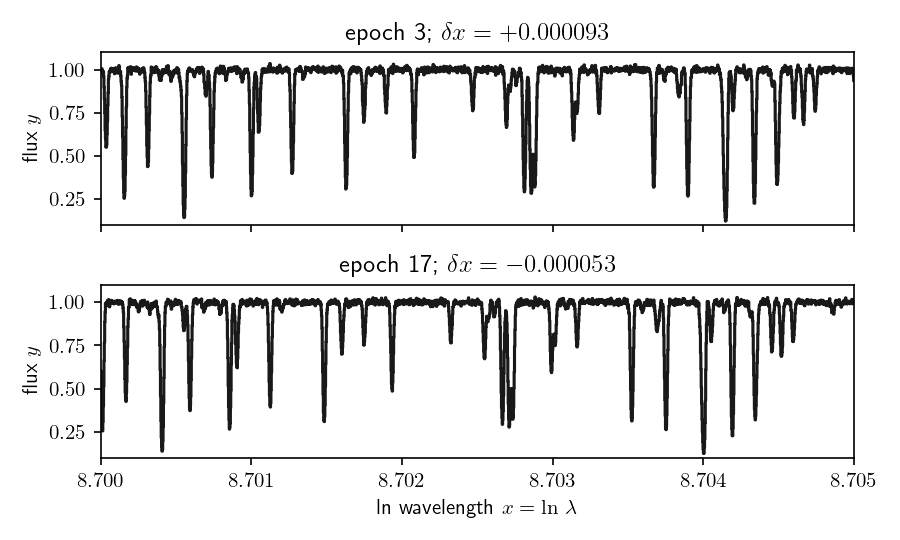
\includegraphics[width=\textwidth]{../notebook/data.png}
    \end{center}
    \caption{Two example toy-data spectra, generated according to the rules described in the main text.
    At each epoch the true spectrum has the same overall shape; the only differences from epoch to epoch are from Doppler-shift changes and shot noise.\label{fig:data}}
  \end{mdframed}
\end{figure}
\begin{figure}[tp]
  \begin{mdframed}
    \begin{center}
    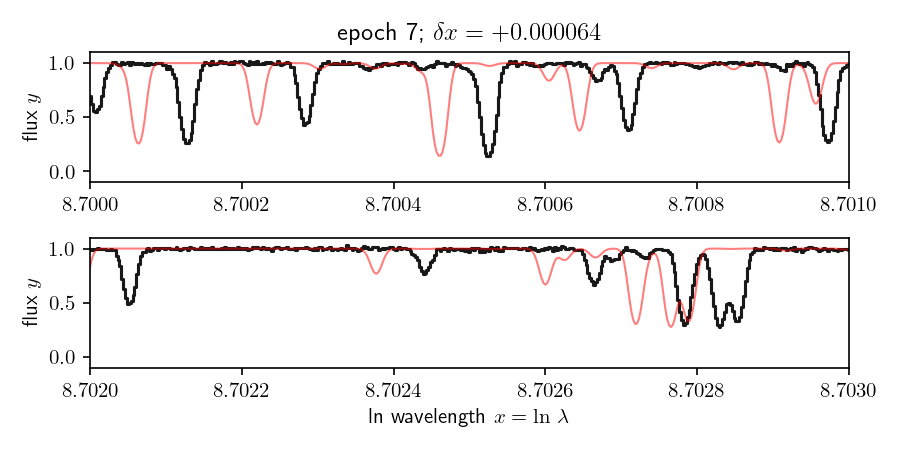
\includegraphics[width=\textwidth]{../notebook/datazoom.png}
    \end{center}
    \caption{A zoom in on one of the toy-data spectra. Shown are both the data (dark black step function) and the true spectral model (thin red smooth line). The data for this epoch is Doppler shifted relative to the model, which is at zero Doppler shift.\label{fig:datazoom}}
  \end{mdframed}
\end{figure}

The toy-data assumptions are unrealistic for an entire extracted spectrum from a present-day spectrograph!
But they are close to appropriate for certain intervals or small segments of spectrum extracted from a high-resolution spectrograph, such as \project{EXPRES} (\citealt{express}):
In small spectral segments, the noise variance (for a bright star) is proportional to the flux, the continuum level is not a strong function of wavelength, the spectrograph resolution is well defined, and the line-spread function is stable.
And indeed, our toy-data simulations span only a small spectral segment.
Importantly, with these toy-data assumptions, we can generate toy data, compute information-theoretic bounds, and test different kinds of radial-velocity estimators.

One detail about these toy data is that although when we generate the noise we use a variance that depends on the true flux expectation, the observer of these data never gets to see that expectation directly.
For this reason, we produce two different noise variance estimates at every pixel:
One is the true noise variance that is related to the true flux expectation and that was used to generate the noise in that pixel.
The other is an empirical noise variance estimate that is based on the observed (noisy) flux in that pixel.
These two noise variances are very similar except in the faintest pixels---that is, the pixels in the centers of strong absorption lines.
In what follows, we use the true noise variances to estimate the information-theoretic bounds.
We use the empirical noise variances in the log-likelihood function (or chi-squared function $\chi^2$) that is used to produce the maximum-likelihood radial velocity estimates.

\figref{fig:mlrvs} shows the true radial velocities for the 64 epochs of toy data, the maximum-likelihood Doppler shifts found by minimizing $\chi^2$ \eqref{eq:chi2}, the residuals, and the information-theoretic (Cram\'er--Rao) bound \eqref{eq:CRLB} derived from the inverse of the Fisher information \eqref{eq:fisher}.
To obtain these radial-velocity estimates the $\chi^2$ function made use of a stellar template, and here we used the exactly correct template--- that is, the template that was used to generate the toy data in the first place.
This figure shows, as expected, that with this use of a perfect template, the minimum-$\chi^2$ radial-velocity estimates, which are maximum-likelihood estimates, saturate the information-theoretic bound.
In \secref{sec:sensitivity}, cross-correlation with a slightly wrong template delivers Doppler shifts that don't saturate the bound.

\begin{figure}[tp]
  \begin{mdframed}
    \begin{center}
    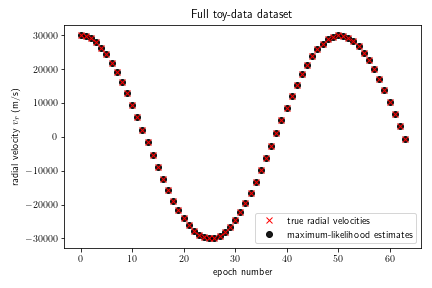
\includegraphics[width=\textwidth]{../notebook/full.png}
    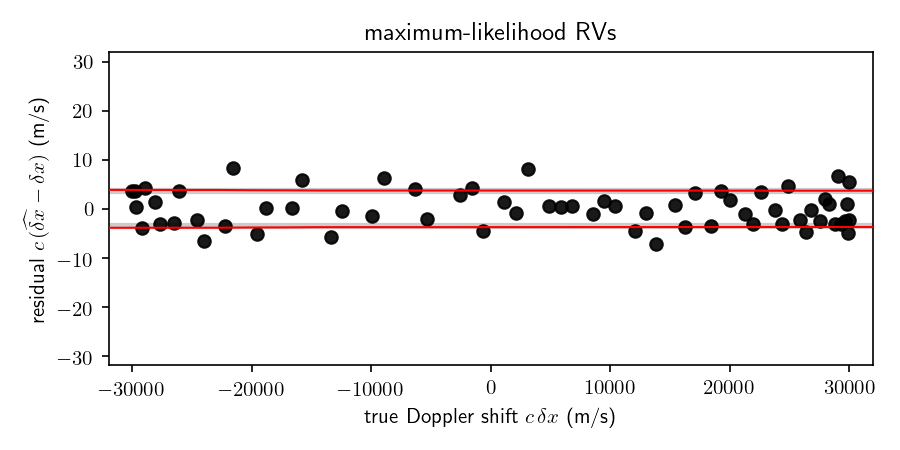
\includegraphics[width=\textwidth]{../notebook/mlrvs.png}
    \end{center}
    \caption{Demonstration that maximum-likelihood estimates saturate the information-theoretic bound.
    The top panel shows both the true doppler shifts for the 64 epochs of toy data and the maximum-likelihood estimates.
    The bottom panel shows the residuals (estimate minus true) as a function of true doppler shift.
    In the bottom panel, the thin red lines indicate the Cram\'er--Rao lower bound on the root-variance (the square-root of the inverse of the Fisher information), and the thick grey lines indicate the 16th and 84th percentiles of the residuals (the empirical one-sigma region).
    The fact that the thin red lines overlap the thick grey lines shows that the maximum-likelihood estimates saturate the information-theoretic bound, as expected.\label{fig:mlrvs}}
  \end{mdframed}
\end{figure}

\section{Cross-correlation}\label{sec:ccf}

Most data-analysis pipelines associated with radial-velocity spectrographs do not explicitly optimize a likelihood function to obtain the radial velocities; nor do they explicitly minimize any kind of chi-squared expression.
Instead they optimize a cross-correlation between the data and a template spectrum.
And yet they deliver excellent radial velocities in general (CITE?).
How is this possible?
It turns out that, under a restrictive set of assumptions, the optimization of a cross-correlation is identical to the optimization of a likelihood function.
Here is the argument:

The estimate $\widehat{\delta x}$ in \eqref{eq:argmin} is a minimum of a $\chi^2$ expression \eqref{eq:chi2}.
The square of the difference in the $\chi^2$ can be expanded as follows
\begin{align}\label{eq:chi2ccf}
    \chi^2 &= \underbrace{\sum_{i=1}^n \frac{y_i^2}{\sigma_i^2}}_{\text{constant}}
         - 2\,\underbrace{\sum_{i=1}^n \frac{y_i\,f(x_i - \delta x)}{\sigma_i^2}}_{\text{like a cross-correlation}}
         +    \underbrace{\sum_{i=1}^n \frac{[f(x_i - \delta x)]^2}{\sigma_i^2}}_{\text{can be made constant}} ~,
\end{align}
where the first term is a constant that doesn't depend on $\delta x$,
the second term is a kind of inverse-variance-weighted cross-correlation between the data $y$ and the template $f(x)$,
and the third term is very close to constant as $\delta x$ varies (and can be made to be exactly constant by suitably normalizing $f(x-\delta x)$).
Thus minimization of a $\chi^2$ (or maximization of a Gaussian likelihood function) is nearly equivalent to maximization of a cross-correlation.
In the covariant-noise case, the cross-correlation becomes something like
\begin{align}
    \sum_{i=1}^n \frac{y_i\,f(x_i - \delta x)}{\sigma_i^2} &\rightarrow \vy^\top\vC^{-1}\,\vf(\delta x)\label{eq:wccf} ~,
\end{align}
but the story is the same---that is, that $\chi^2$ minimization is equivalent to cross-correlation maximization.
Technically a cross-correlation function is defined by an integral, not a sum!
These are the same when the argument of the sum is weighted by the a pixel measure (typically a pixel width) and the pixel measures  go to zero.
The terms in \eqref{eq:wccf} constitute precisely a cross-correlation with an inverse-variance measure in the $x$ space, in the limit that the pixel spacing is tiny.

In the expansion \eqref{eq:chi2ccf}, there are three terms, one is a constant (doesn't depend on the Doppler shift $\delta x$), and one is marked ``can be made constant''.
It turns out that for precise radial-velocity measurement, it is essential that this term be made constant.
The reason it isn't precisely constant under uncontrolled conditions is that as the Doppler shift changes, some absorption lines at the edges of the spectral range enter and leave the domain.
These change slightly the auto-correlation of the template $f(x)$ with itself, when this auto-correlation is restricted (as it is) to the domain of the observed data segment.
Thus it is imperative that the template be renormalized at every Doppler shift by a normalization that looks like this:
\begin{align}
    f(x_i-\delta x) &\leftarrow f(x_i-\delta x)\,\left[\sum_{i=1}^n \frac{[f(x_i-\delta x)]^2}{\sigma_i^2}\right]^{-1/2} ~.
\end{align}
With this Doppler-shift-dependent normalization, the auto-correlation term in the expansion \eqref{eq:chi2ccf} becomes precisely constant with $\delta x$.
This might seem like a detail, but in our toy-data example, failure to renormalize in this manner introduces structured scatter in the radial-velocity estimates far in excess of the information-theoretic bound. 

A variation of this effect in action may be seen in the HARPS spurious one-year signals diagnosed by \citet{Dumusque2015}, where the seasonal barycentric shifts of certain spectral features in and out of CCD stitching boundaries on the HARPS detector effectively introduced a seasonal variability to the normalization. 
This is a subtle case in which the the lines are not actually leaving the wavelength domain of the data, but instead are moving through a wavelength region that is affected by quantum efficiency (QE) variations. 
Ideally this effect would be encoded in the uncertainty $\sigma_i$ of the pixels known to be affected by QE variations, or else perhaps added to a forward model for the data at the extraction step, if it leads to a predictable bias.
Detailed discussion of such a model is out of scope here.

Many data pipelines do a simple unweighted cross-correlation, not weighted by the inverse pixel variances $1/\sigma_i^2$ (nor the inverse covariance matrix $\vC^{-1}$).
Technically maximization of the simple unweighted cross-correlation function is not equivalent, but for much of the spectrum, it won't be very different, because much of the spectrum has uncertainties that lie in a reasonably low dynamic-range band, for the most part.
And besides, in a typical present-day high-resolution spectrograph, the cross-correlation function is an average over hundreds of thousands of pixels, so local variations in the pixel variances aren't extremely important to the final answer, especially if very noisy parts of the spectrum have been censored or masked out.

In terms of detailed implementation, one interesting and perhaps surprising fact is that it is not necessary to do very fine steps in the Doppler shift $\delta x$ when numerically optimizing this cross-correlation.
The reason is that if the data are taken with a spectrograph with well-defined resolution $R$, there can't be sharp features in the cross-correlation function at scales $\Delta(\delta x)<1/R$.
The Doppler shift $\delta x$ can be scanned on a grid that is, say $1/(3R)$ and then the 3 pixels in the empirical cross-correlation peak can be fit with a parabola; the optimal estimate $\widehat{\delta x}$ of the Doppler shift $\delta x$ is the maximum of that parabola.
This is illustrated in \figref{fig:ccf}.

\begin{figure}[tp]
  \begin{mdframed}
    \begin{center}
    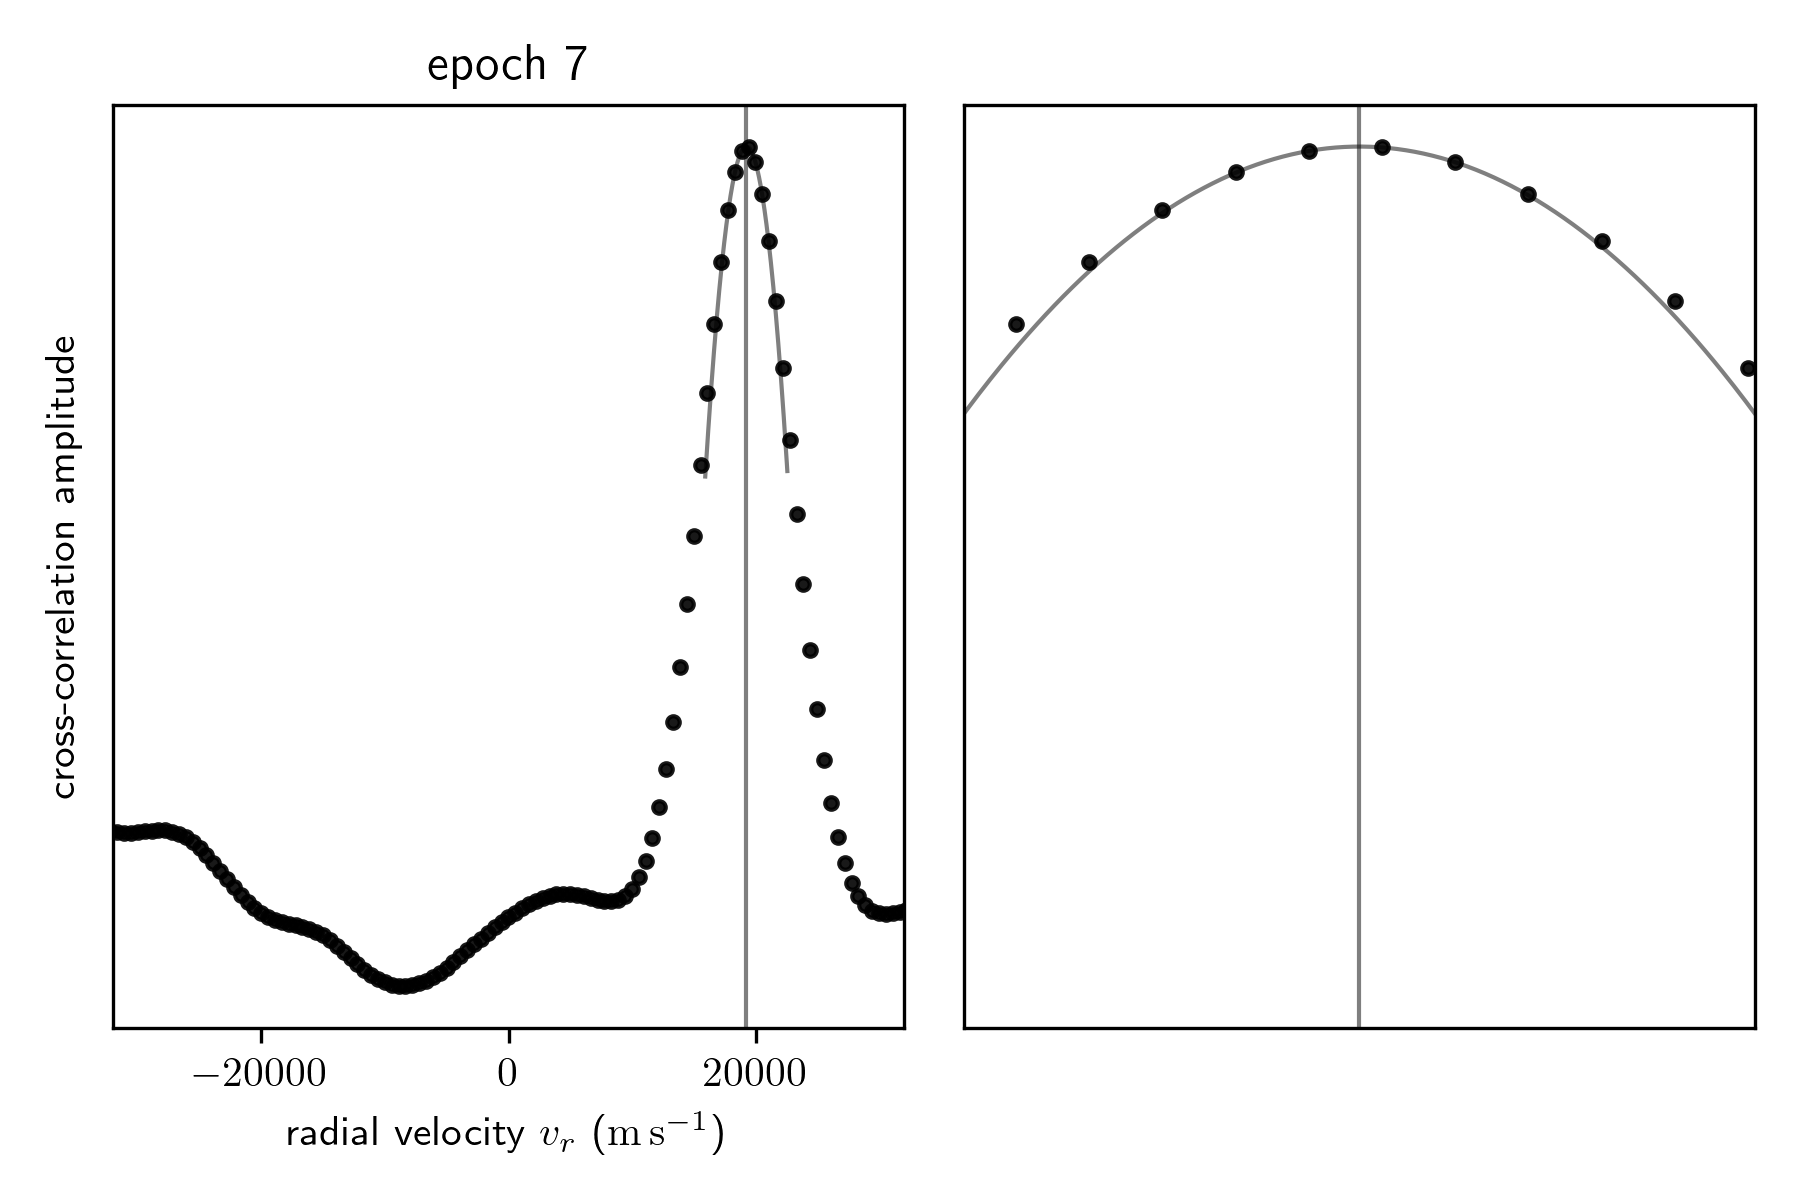
\includegraphics[width=\textwidth]{../notebook/ccf.png}
    \end{center}
    \caption{Optimizing a function with the parabola trick. The left panel shows the cross-correlation amplitude (data cross-correlated with a correct template spectrum) measured at a discrete set of Doppler shifts. The right panel shows a zoom in on the peak. The smooth parabola is fit to the three peak values of the cross-correlation function, and the vertical line shows the optimum of that parabola.\label{fig:ccf}}
  \end{mdframed}
\end{figure}

The cross-correlation radial-velocity measurement precision on the full toy-data dataset is shown in \figref{fig:ccfrvs}.
As expected, these radial-velocity estimates also saturate the information-theoretic bound.

\begin{figure}[tp]
  \begin{mdframed}
    \begin{center}
    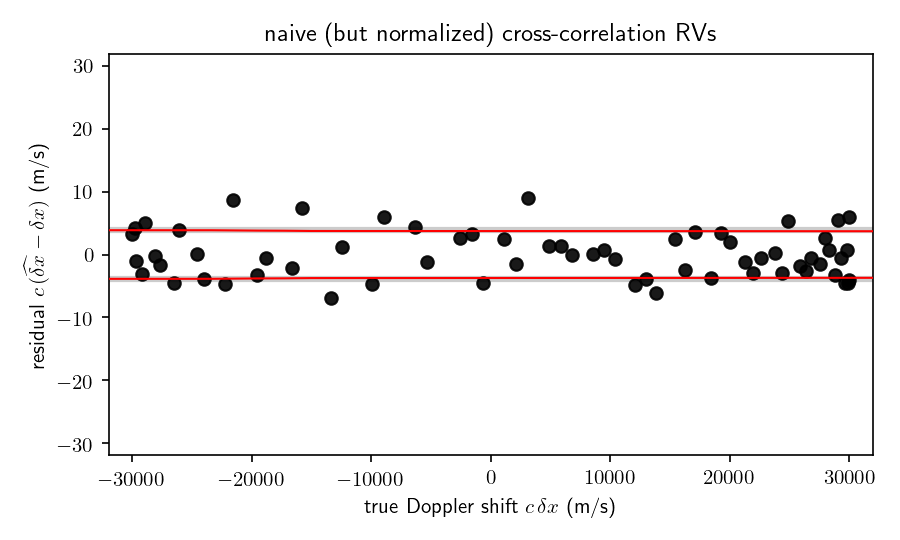
\includegraphics[width=\textwidth]{../notebook/ccfrvs.png}
    \end{center}
    \caption{Same as the bottom panel of \figref{fig:mlrvs}, but for the cross-correlation Doppler-shift estimates. The coincidence of the thin red and thick grey lines shows that the cross-correlation estimates saturate the information-theoretic bound.\label{fig:ccfrvs}}
  \end{mdframed}
\end{figure}

For both the cross-correlation radial-velocities in this \sectionname{} (\figref{fig:ccfrvs}) and the maximum-likelihood radial-velocities shown in \secref{sec:data} (\figref{fig:mlrvs}), it was essential that the template spectrum $f(x)$ be accurate, or accurately represent our expectation for the spectrum.
When the template spectrum does not look like the true spectrum, both biases and additional variance are introduced.
A full description of this is out of scope, but we show one particular example below in \secref{sec:binary} (\figref{fig:wrongbccfrvs}).

\section{Binary mask magic}\label{sec:binary}

In this \sectionname{} we discuss a technical matter relevant to present-day radial-velocity pipelines.
This point is a slight digression to the main information-theory thread, but it is relevant to understand why present-day pipelines work well.

We demonstrated, above, that maximum-likelihood or cross-correlation with a good spectral template leads to information-theoretic optimal estimates of radial velocity.
However, in many present-day operating instrument pipelines (CITE) in fact the extracted spectrum is instead cross-correlated with a \emph{binary mask} (for example, \citealt{pepe}; CITE OTHERS).
This is a function with values somewhere between zero and one in small wavelength regions that correspond to a select subset of stellar absorption lines, and values of zero at all other wavelengths. 
It is far from obvious that this method, which appears to `fit' a spectrum with an extremely un-spectrum-like function, should deliver radial velocities that saturate any bounds!
And yet binary mask based pipelines \emph{do} produce excellent estimates of radial velocity.

How can we understand this?
One thing to note: because the binary mask, in some sense, indicates the \emph{negative} of the absorption, the cross-correlation is more-or-less \emph{minimized} at the correct radial velocity, not maximized.
Secondly, the way the cross-correlation is used in these pipelines is not that it is directly minimized, but instead the dip in the cross-correlation function is \emph{fit with a smooth model} (usually an inverted Gaussian function).
The radial-velocity measurement is then derived as the best-fit Gaussian mean.
This procedure is functionally equivalent to convolving the binary mask with a Gaussian---thus making a reasonably good template for the spectrum---and then optimizing the cross-correlation of the data with that good (no longer binary) template. 
Importantly, the order of operations in the standard binary mask procedure means that the equivalent Gaussian convolution is done with the optimal Gaussian for the observed spectrum.
In what follows, we demonstrate this quantitatively.

Imagine that you have a binary mask function $\beta(x)$ with the beautiful property that if you smooth it with some line-spread function $\psi(x-x')$ it becomes a reasonable model template $y(x)$ for the deviation of the spectrum from the continuum.
Think of the binary mask as being (effectively) an absorption line list, with the width of each binary line in the binary mask corresponding to the equivalent width the line has in the spectrum.
Then convolution with a model $\psi(x-x')$ of the line-spread function will give a model for the finite-resolution spectrum.
That is, imagine that we have a binary mask $\beta(x)$ and kernel function $\psi(x-x')$ such that
\begin{align}
    y(x) &= 1 - \int\beta(x')\,\psi(x-x')\,\dd x' ~,
\end{align}
where $y(x)$ is now a good spectral template, and the $1$ represents the continuum level of that template.
Now pixelize the binary mask, the line-spread function, and the data onto an extremely fine pixel grid.
The convolution becomes
\begin{align}
    f_i &= 1 + \sum_{i'=-k}^k \beta_{i-i'}\,\psi_{i'} ~.
\end{align}
Now the cross-correlation function of the data with this numerically constructed template $f$ can be written as a cross-correlation of the data with the binary mask $b$, subsequently cross-correlated with the the kernel $\psi$.
This, in turn, will be optimized at the same place as a fit of the kernel $\psi$ to the cross-correlation between the data and the binary mask.
In equations (HOGG SAYS: I THINK THERE'S a sign error here):
\begin{align}
    \CCF(\delta; f) &= \sum_{i=1}^n \frac{y_i}{\sigma_i^2}\,\sum_{i'=-k}^k \beta_{i-\delta-i'}\,\psi_{i'} + \text{const}\\
    &= \sum_{i'=-k}^k \CCF(\delta+i';\beta)\,\psi_{i'} + \text{const}\\
    &= -\frac{1}{2}\sum_{i'=-k}^k [\CCF(\delta+i';\beta) - \psi_{i'}]^2 - \text{const}\mbox{~(s.t. conds.)}\\
    \arg\max_{\delta} \CCF(\delta; f) &= \arg\min_{\delta} \sum_{i'=-k}^k [\CCF(\delta+i';\beta) - \psi_{i'}]^2 ~,
\end{align}
where $\CCF(\delta; f)$ is the cross-correlation of the data with the template $f$ at (pixel level) Doppler shift $\delta$,
$\CCF(\delta, \beta)$ is the same but for the binary mask $b$,
and in the final step we use the above-mentioned fact that maximization of a cross-correlation is equivalent to minimization of a $\chi^2$.
Thus even though optimization of the binary-mask cross-correlation function $\CCF(\delta; b)$ would not come close to saturating the information-theoretic bounds on the measurement of the Doppler shift, least-square fitting of that cross-correlation function with a model of the line-spread function will come close to saturating it. 
It is necessary that a sufficiently large span of the CCF be fit with the line-spread function to constrain the line-spread-function fit and extract the maximum information.
That is, the parabola trick discussed in \secref{sec:ccf} would produce very noisy estimates here (and therefore not saturate any bound).

HOGG: BEDELL say: We should test this ``sufficiently large'' claim and make it specific? Like plot the RMS vs the size of the fitting region?

In this \sectionname{} we are being a bit loose with the sums over pixels $i$:
Because the binary mask involves very fine structure in the $x$ space, in practice these sums must either be performed on a very fine pixel grid (much finer than natural extraction grids for real spectrographs), or else the data must be interpolated onto the features of the binary mask.
In practice most real pipelines do the latter, we believe.
The binary-mask cross-correlations we compute here (below) are computed by interpolating (with a cubic spline interpolator) the data $y_i$ onto the non-zero parts of the binary mask and then integrating over the small binary-mask windows.

In the toy-data system, we made the binary mask by processing the list of true line locations and true line equivalent widths that was used to make the true spectral expectation (\secref{sec:data}).
The binary mask is set to zero everywhere except in a set of non-zero windows, one centered on each true line above an equivalent width limit of $10^{-6}$ in ln-wavelength units.
Each window gets a width that is $1/4$ of the true line equivalent width.
Windows are deleted if they are within Doppler shifts of $\pm 40\,\kmps$ of either edge of the observed spectral range, so that there are no difficult edge effects (at some loss of spectral features).
Windows that overlap are combined by adopting width-weighted average locations and adding the widths.
The binary mask created this way is visualized in \figref{fig:binarymask}.

\begin{figure}[tp]
  \begin{mdframed}
    \begin{center}
    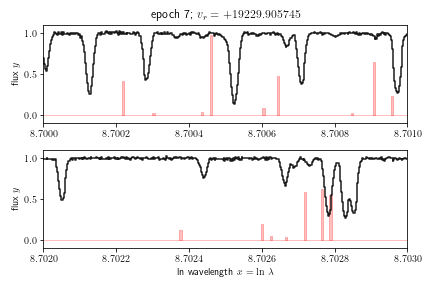
\includegraphics[width=\textwidth]{../notebook/binarymask.png}
    \end{center}
    \caption{A visualization of part of the binary mask. The dark black step function shows the same spectral segment shown in \figref{fig:datazoom}, but the light red filled step function shows the binary mask employed in the text, Doppler shifted to the correct Doppler shift for this epoch. Note that the binary mask is zeroed out in a segment at the left edge of the top plot; this is a result of the censoring of lines that might Doppler shift in and out of the observed spectral range.\label{fig:binarymask}}
  \end{mdframed}
\end{figure}

\figref{fig:bccfrvswrong} shows that the cross-correlations of the binary mask with the toy spectral data by themselves deliver radial-velocity estimates that don't come close to saturating the information-theoretic bound.
That's not surprising; the maximum-likelihood and cross-correlation radial-velocity estimates are only efficient when the spectral template is an accurate representation of the spectral expectation.
However, \figref{fig:bccfrvs} shows how the radial-velocity estimates improve when the binary-mask cross-correlation functions are subsequently fit with a Gaussian that looks like the line-spread function.
These post-processed binary-mask results do saturate the bound.

\begin{figure}[tp]
  \begin{mdframed}
    \begin{center}
    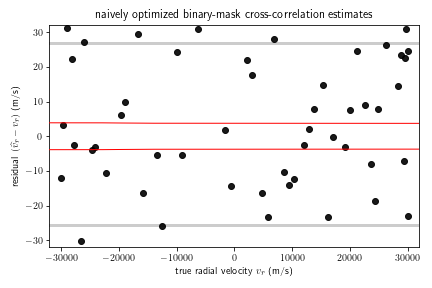
\includegraphics[width=\textwidth]{../notebook/bccfrvswrong.png}
    \end{center}
    \caption{Same as the bottom panel of \figref{fig:mlrvs} but showing the results of naively optimizing the cross-correlation of the data with the binary mask. These estimates do not saturate the information-theoretic bound because the binary mask is not a good representation of the spectral expectation.\label{fig:bccfrvswrong}}
  \end{mdframed}
\end{figure}%
\begin{figure}[tp]
  \begin{mdframed}
    \begin{center}
    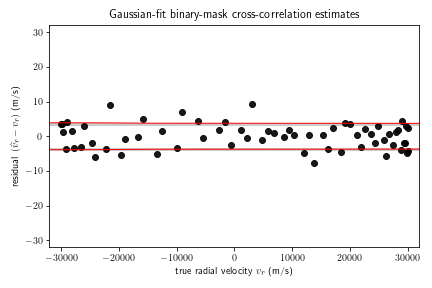
\includegraphics[width=\textwidth]{../notebook/bccfrvs.png}
    \end{center}
    \caption{Same as the bottom panel of \figref{fig:mlrvs} but showing the results of optimizing the fit of a Gaussian function to the cross-correlation of the data with the binary mask. Compare this with \figref{fig:bccfrvswrong}. Binary-mask cross-correlation functions deliver bound-saturating Doppler-shift estimates when fit after the fact with a Gaussian function. See text for discussion.\label{fig:bccfrvs}}
  \end{mdframed}
\end{figure}

Experiments suggest that the binary-mask operations are very sensitive to edge effects.
In making the mask, we removed lines near the edges of the observed spectral range, so that our results aren't contaminated by variations resulting from lines entering and leaving the spectral range.
This probably leads to a small loss in precision, but the results saturate the information-theoretic bound nonetheless.

\section{Empirical spectral templates}\label{sec:templates}

The most important thing about radial-velocity variations with time---for a star with a constant intrinsic spectrum---is that the variations can be measured empirically, without any fundamental physical beliefs about the star (other than its lack of intrinsic variability).
That is, the investigator does not need to approach the problem with a good-fitting theoretical stellar spectral template $f(x)$.
The spectral template $f(x)$ can be derived directly from the observations of the star themselves.
The requirement here is that there be substantial numbers of epochs of observations, sufficient to provide an estimate of the mean spectrum that is (much) higher in signal-to-noise than the spectral data at any individual epoch.
This realization is the fundamental motivation for the \wobble{} project (\citealt{wobble}).

There is a simple argument about the quality of empirical templates that goes as follows:
Imagine that you have $N$ epochs of observation of a star, all with the same spectrograph, and each of these observations is at similar signal-to-noise ratio.
If the star does not vary epoch-to-epoch, an empirical spectral template will accurately describe the spectrum of the star in this spectrograph (by assumption and construction), and it will have a signal-to-noise ratio that is on the order of $\sqrt{N}$ larger than the signal-to-noise of any individual epoch.
The use of the empirical template will add in quadrature to any individual-epoch Doppler-shift uncertainty a template-origin uncertainty that is smaller by a factor of $\sqrt{N}$.
Once $N$ is large enough---and because this additional noise adds only in quadrature---the empirical template ought to be as good (or better, since a certain kind of accuracy is guaranteed) as any theoretical spectral template for the determination of Doppler shifts.
In the toy data we use here (\secref{sec:data}), $N=64$.

Empirical templates can be created by interpolating spectra to a common logarithmic wavelength grid and averaging.
Interpolations wwre performed with cubic splines.
With an empirical template in hand, cross-correlation doppler shifts can be estimated, updating the beliefs about the spectra rest frames, and then the templates can be re-made.
This process can be iterated to convergence.
In this process, the initialization matters.
In making the results in this \sectionname, we initialized at the wrong binary-mask results shown in \figref{fig:bccfrvswrong}, not at good radial-velocities, and yet the results are excellent.
That is, we didn't cheat.
We show the empirical template in \figref{fig:empirical} and we show the
empirical-spectrum cross-correlation radial-velocity results in \figref{fig:empiricalrvs}

\begin{figure}[tp]
  \begin{mdframed}
    \begin{center}
    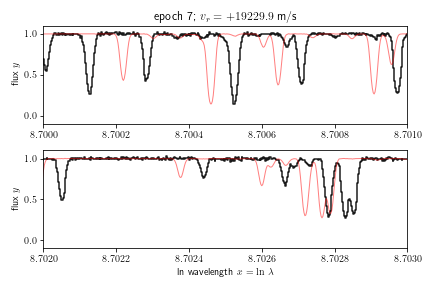
\includegraphics[width=\textwidth]{../notebook/empirical.png}
    \end{center}
    \caption{A visualization of part of the empirical spectral template. The dark black step function shows the same spectral segment shown in \figref{fig:datazoom}, but the thin red smooth line now shows not the true spectral template but instead the empirical template obtained by shifting and averaging the observed data. Note that the empirical template constructed here has no lines in a segment at the left edge of the top plot; this is a result of the censoring of spectral regions that might Doppler shift in and out of the observed spectral range.\label{fig:empirical}}
  \end{mdframed}
\end{figure}
\begin{figure}[tp]
  \begin{mdframed}
    \begin{center}
    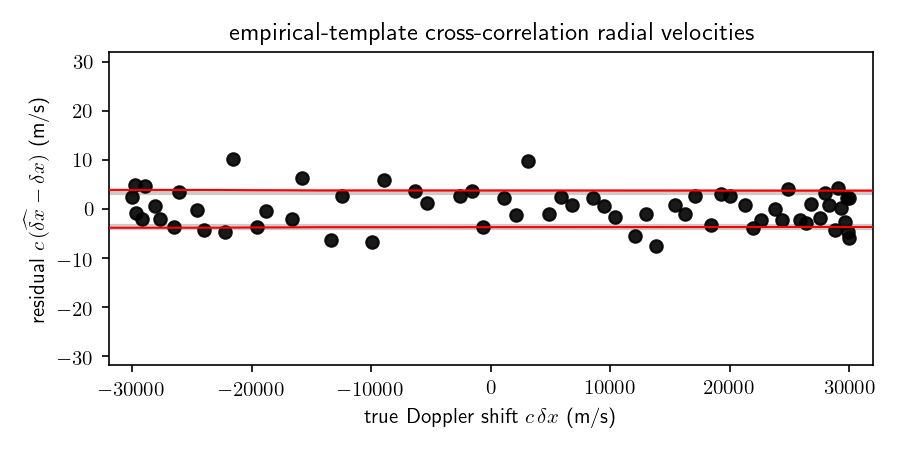
\includegraphics[width=\textwidth]{../notebook/empiricalrvs.png}
    \end{center}
    \caption{Same as the bottom panel of \figref{fig:mlrvs} but showing the results of optimizing the cross-correlation of the data with an empirical template made from the epoch data themselves. Compare with \figref{fig:ccfrvs}; this shows that empirical templates are just as good as true templates; they both saturate the information-theoretic bounds. When empirical templates are used, the zero-point of the Doppler shifts becomes ambiguous; in order to make this plot, the mean of the residuals was subtracted from all of the residuals.\label{fig:empiricalrvs}}
  \end{mdframed}
\end{figure}

The empirical template can be subject to issues at its edges, since each spectral epoch reveals a slightly different stellar rest-frame spectral range in a spectrograph of fixed spectrograph-frame spectral range.
For this reason, when we made the spectral template, we zeroed out (or really set to unity) the empirical spectra in a logarithmic wavelength range that is within $40\,\kmps$ of either edge of the template spectral range.
Evidence of this censoring is visible in \figref{fig:empirical}.

One interesting question that arises in the use of empirical templates is whether the inclusion of a particular epoch in the template biases the Doppler measurement made \emph{at that epoch}.
In the results shown in \figref{fig:empiricalrvs} this effect was removed in the sense that each epoch's Doppler shift was obtained by cross-correlation with a template constructed from the average of all \emph{other} epochs.
That is, the cross-correlations were with leave-one-out empirical templates.
Experiments suggest that, for the 64-epoch toy data set here, the self-use bias is very small.
But it might be significant when there are many fewer epochs.

In the Doppler-shift estimation methods in the previous \sectionname s, the template or likelihood was based on a theoretical model of the star.
Thus the template can be made at zero Doppler shift (zero velocity) and the measured Doppler shift is relative to this zero.
In the case of empirical templates, this is no longer possible.
There is no indication or sense of the true zero of velocity (for very deep reasons!).
In the iterative procedure used here to converge the template and the Doppler shifts, the effective zero-point of the Doppler shifts can (and does) shift.
In making \figref{fig:empiricalrvs}, we removed this shift by setting the mean Doppler-shift residual to zero.

\section{Sensitivity to assumptions}\label{sec:sensitivity}

We opened (\secref{sec:assumptions}) with a long list of restrictive assumptions.
Here we perform experiments in which we make the data weakly incompatible with some of these assumptions and look at how the radial-velocity measurements are affected.
These experiments are not intended to exhaustively test any of the assumptions; they are just demonstrations that the assumptions do indeed matter.

\paragraph{Wavelength-calibration issues}
As stated in \secref{sec:assumptions}, in everything above we assumed that the spectra are perfectly calibrated in a wavelength sense.
This means that every extracted spectral pixel $i$ has an accurate associated logarithmic wavelength value $x_i$.
In practice, the wavelengths of the extracted pixels are themselves noisy measurements based on noisy calibration data, and thus this assumption must be wrong in detail.
In addition to the noise in calibration data, there can also be wavelength-calibration issues because detectors are real devices with non-uniformities in their pixel positions (see, for example, \citealt{excalibur}); these non-uniformities are not captured in all calibration methods.

In order to explore wavelength-calibration issues, we make data as per \secref{sec:data} but instead of having the data on a regular wavelength grid, we perturb the wavelength grid with a sinusoidal perturbation.
This perturbation is sinusoidal in $x$, has exactly zero mean $x$ shift, and is different in amplitude for every epoch.
The perturbations have amplitudes on the order of 0.1~pixels, peak-to-peak.
Doppler shifts are measured in these distorted toy spectral data using the template cross-correlation as in \secref{sec:ccf}.

The results are shown in \figref{fig:calibration}, which can be compared to the baseline results shown in \figref{fig:ccfrvs}.
The wavelength perturbations increase the empirical scatter in the measurements, such that they no longer saturate the information-theoretic bound.
It is interesting to note that this systematic wavelength-calibration noise contaminates the Doppler-shift measurements despite the fact that the introduced noise has, in itself, no net or mean shift in the logarithmic-wavelength $x$ space.

\begin{figure}[tp]
  \begin{mdframed}
    \begin{center}
    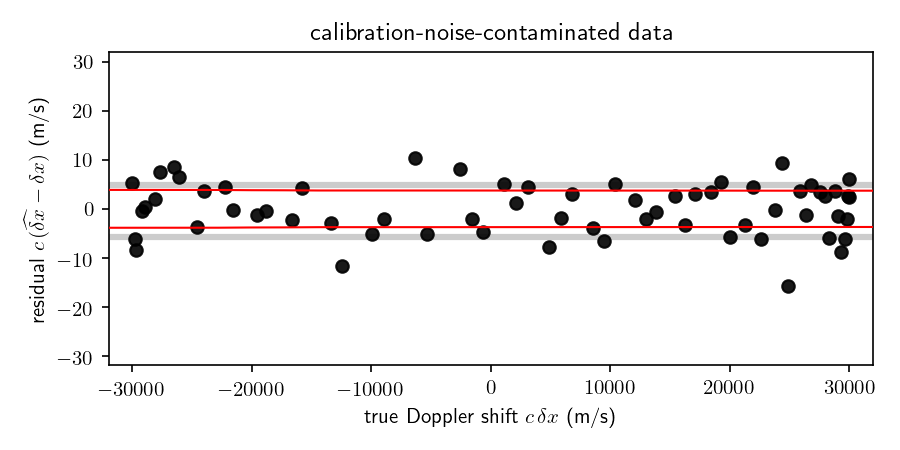
\includegraphics[width=\textwidth]{../notebook/calibration.png}
    \end{center}
    \caption{Same as \figref{fig:ccfrvs} but now showing cross-correlation results after systematic wavelength-calibration issues are introduced. The calibration issues are below the one-thousandth-of-a-pixel level and have no net Doppler shift (see text).\label{fig:calibration}}
  \end{mdframed}
\end{figure}

\paragraph{Unmodeled low-amplitude telluric lines}
As stated in \secref{sec:assumptions}, in everything above we assumed that telluric lines either don't exist, or else are handled properly.
Telluric lines can be handled by fitting and subtracting them, or by masking the data at their locations.
However, it is possible for there to be tiny, unknown telluric features that affect the data but aren't either known or individually detectable.
The possible existence of these lines was one of the motivations for the \textsl{wobble} project (\citealt{wobble}.

Here we test the sensitivity to unmodeled telluric contamination by creating a substantial number of very low amplitude absorption lines and combining them into a telluric template, much as we create the spectral template above in \secref{sec:data}.
The telluric template created this way is shown in \figref{fig:telluric}.
It only contains low-amplitude variations that would not be clearly visible at any epoch.
The spectral data are multiplied by this telluric template to (approximately) simulate contamination by weak telluric lines.
Importantly, although the spectral data are at different Doppler shifts relative to the spectrograph wavelength grid, the telluric component is always at zero Doppler shift because it is assumed to be fixed with respect to the atmosphere, which is assumed to be fixed relative to the spectrograph.

Doppler shifts are measured in these telluric-contaminated data using the template cross-correlation as in \secref{sec:ccf}.
The results are shown in  \figref{fig:telluric}, which can be compared to the baseline results shown in \figref{fig:ccfrvs}.
The introduction of telluric contamination increases the empirical scatter in the measurements, such that they no longer saturate the information-theoretic bound.

\begin{figure}[tp]
  \begin{mdframed}
    \begin{center}
    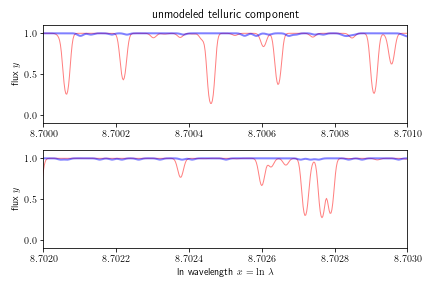
\includegraphics[width=\textwidth]{../notebook/telluricmodel.png}
    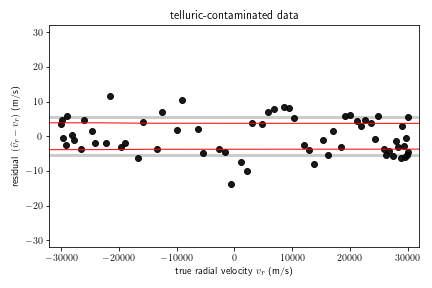
\includegraphics[width=\textwidth]{../notebook/telluric.png}
    \end{center}
    \caption{The top panels show the introduced telluric effect in a thick blue line, in comparison with the true spectral template (thin red line, repeated from \figref{fig:datazoom}). The telluric template (thick blue) stays fixed in logarithmic wavelength $x$ while the spectral template (thin red) Doppler shifts. The bottom panel is the same \figref{fig:ccfrvs} but now showing cross-correlation results after this unmodeled telluric contamination is introduced.\label{fig:telluric}}
  \end{mdframed}
\end{figure}

\paragraph{Small spectral variations}
As stated in \secref{sec:assumptions} (and even our title), in everything above we assumed that the star is non-variable. That is, the only differences from epoch to epoch are the Doppler shift and the photon noise.
There are no variations in spectral shape, line strengths, line positions, line-spread function, or line ratios.
Performing good Doppler-shift measurement in the presence of arbitrary spectral variability is out of scope here; it is the subject of an important future line of research.
Here we just look at one simple kind of variability: Variable line strengths.

Variable spectral data are made as in \secref{sec:data} but instead of using the identical spectral template for every simulated epoch, the equivalent widths of the lines are varied fractionally by small fractions such that there is a one-percent scatter in the line equivalent widths.
Everything else about the data generation is left unchanged.
These spectral variations do not involve moving any lines to shorter or longer wavelengths, they only involve the line \emph{strengths}.

Doppler shifts are measured in these toy time-variable spectral data using the template cross-correlation as in \secref{sec:ccf}.
The results are shown in \figref{fig:variable}, which can be compared to the baseline results shown in \figref{fig:ccfrvs}.
The line-strength variations increase the empirical scatter in the measurements, such that they no longer saturate the information-theoretic bound.
This demonstration can also be seen as a demonstration that cross-correlation with a slightly-wrong spectral template will not saturate the information-theoretic bound.
It is interesting to note that this toy spectral variability contaminates the Doppler-shift measurements despite the fact none of the spectral lines is moved in wavelength.

\begin{figure}[tp]
  \begin{mdframed}
    \begin{center}
    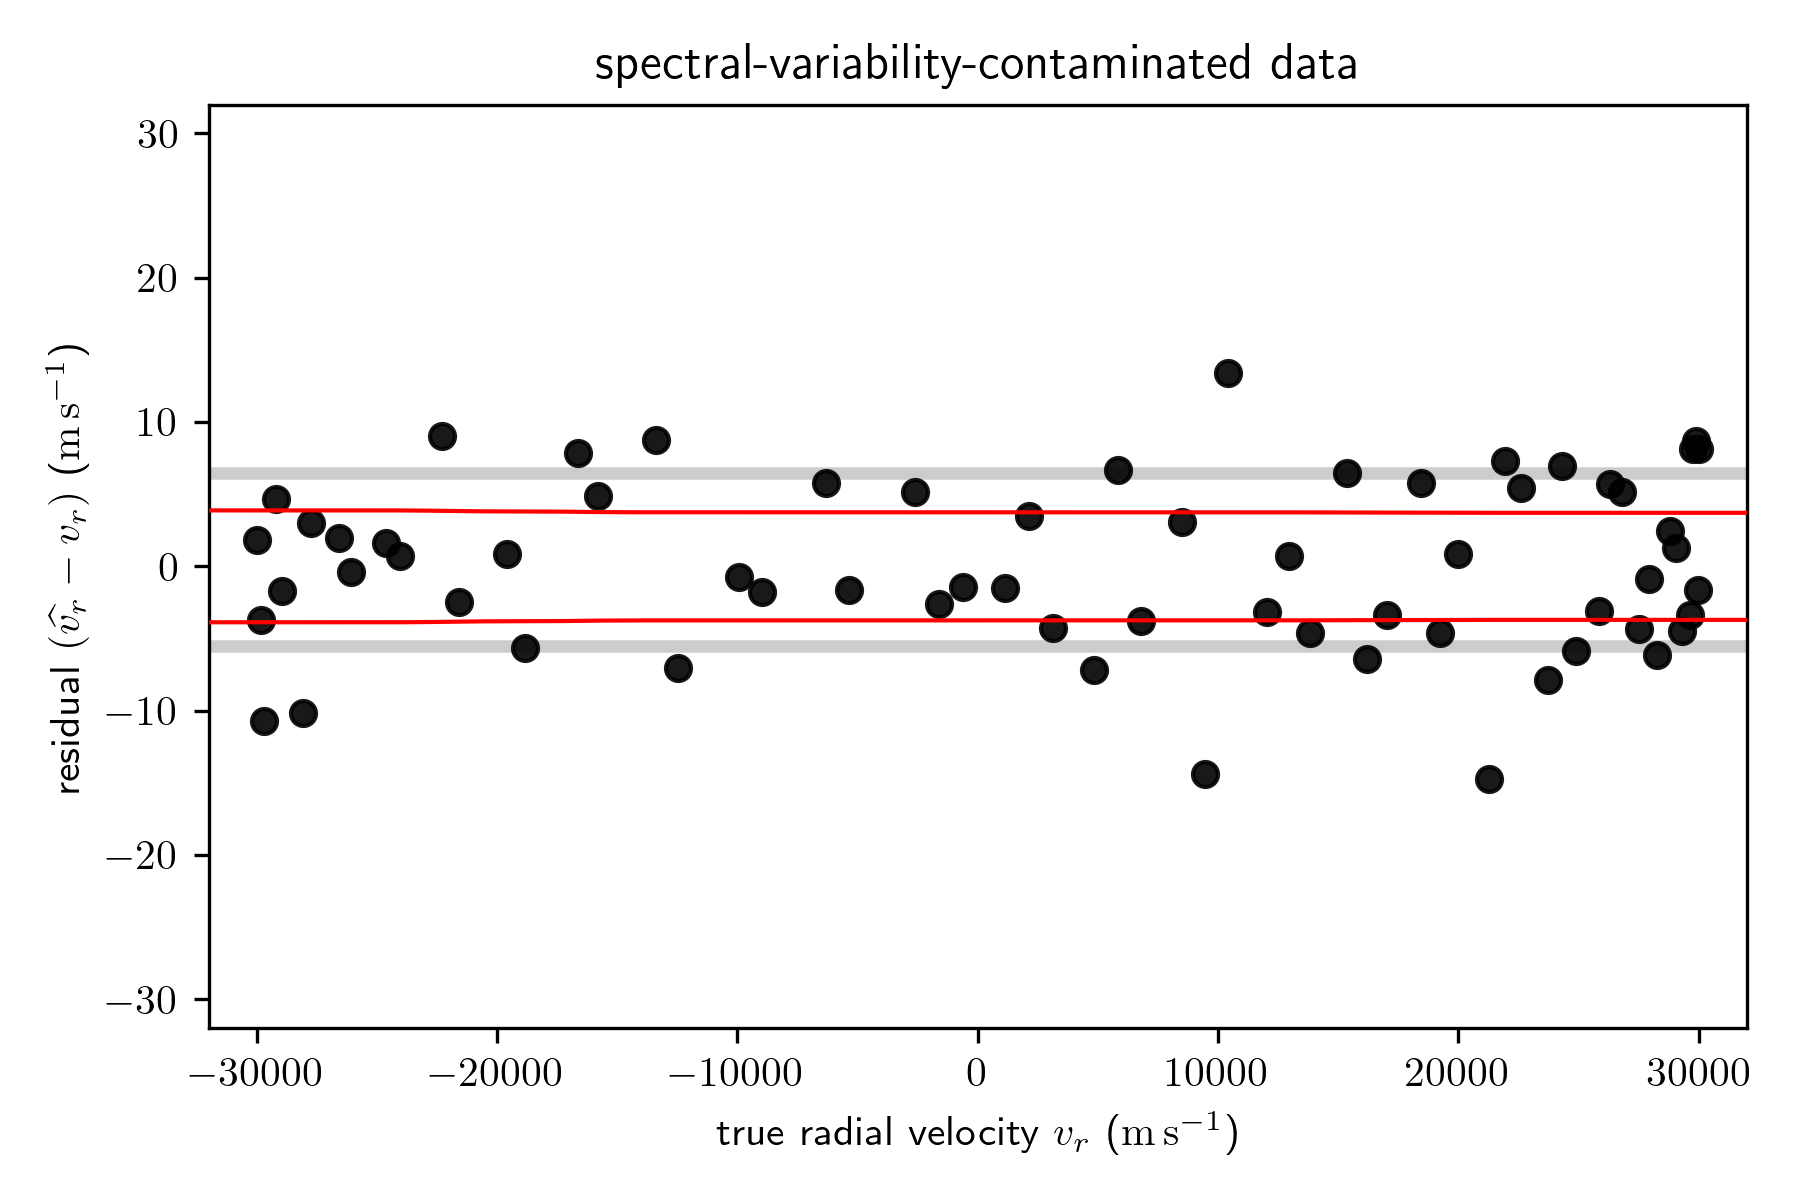
\includegraphics[width=\textwidth]{../notebook/variable.png}
    \end{center}
    \caption{Same as \figref{fig:ccfrvs} but now showing cross-correlation results after spectral variability is introduced. The variability is at the percent level in equivalent widths, only in the line equivalent widths, and not at all in line locations (see text). Nonetheless, the Doppler shift e\label{fig:variable}}
  \end{mdframed}
\end{figure}

\section{Discussion}\label{sec:discussion}

HOGG: What, roughly, is most important about the above?

- Info theory precision result. Contextualize with existing formulations. All is well here.

- Do different methods saturate this bound? Yes, yes they can and do; we have choices.

- Under conditions, the in-practice binary-mask method is a good method; that is, current pipelines probably do saturate the bound. BUT this result depends on strong assumptions (list here!); we elucidate that. mask convolved with gaussian is good; line EWs; LSF; etc.

- We don't test all our myriad assumptions, but the ones we do test appear to be significant; there is a possible full flow-down. Cite Halverson here.

HOGG: How do our quantitative results on our toy data relate to quantitative results on a real star? It's complicated because it depends on the real lines and the spectral coverage (and resolution and so on).

HOGG: Do any of the assumptions change in the face of new technology, new spectrographs, etc? Discuss them at least briefly, and what happens if you want to weaken them. Ground vs space? Cite NASA peeps.

HOGG: Contextualize this work in general RV science (beyond EPRV): What about ACCURATE RV?? What about single-epoch? What about low-R spectrographs? (Call out Gaia here!?) 

HOGG: In the above, make sure to comment on the conceptual point of whether you are measuring a velocity wrt the spectrograph, or a velocity wrt the Solar-System barycenter (as EXPRES does). This distinction is important to the design of extraction pipelines, but doesn't change any of our story here.

HOGG: Then further contextualize in terms of what is done with the RVs after. Perhaps make the point that if you do anything with priors, people can't use the RVs in all the ways they might think that they can?!

HOGG: Do the time-invariant spectrum assumption last and discuss the different possible approaches to this problem. Many of these are being pursued! Cite everyone.

\software{
\project{numpy} \citep{numpy} ---
\project{matplotlib} \citep{matplotlib} ---
\project{scipy} \citep{scipy}
}

\begin{acknowledgments}
It is a pleasure to thank
  Jacob Bean (Chicago),
  John Brewer (SFSU),
  Matthew Daunt (NYU),
  Dan Foreman-Mackey (Flatiron),
  Ben Montet (UNSW),
  Adrian Price-Whelan (Flatiron),
  Hans-Walter Rix (MPIA),
  Julian Stuermer (Uni Heidelberg),
  Lily Zhao (Flatiron),
and the Astronomical Data Group at the Flatiron Institute for valuable discussions and input.
MB thanks the Max-Planck-Institut f\"ur Astronomie in Heidelberg
for hospitality during a critical phase of this project.
\end{acknowledgments}

\begin{thebibliography}{dummy}
  \bibitem[Bedell et al.(2019)]{wobble} Bedell, M., Hogg, D.~W., Foreman-Mackey, D., et al.\ 2019, \aj, 158, 164. doi:10.3847/1538-3881/ab40a7
  \bibitem[Blackman et al.(2019)]{berv-lambda} Blackman, R.~T., Ong, J.~M.~J., \& Fischer, D.~A.\ 2019, \aj, 158, 40. doi:10.3847/1538-3881/ab24c3
  \bibitem[Dumusque et al.(2015)]{Dumusque2015} Dumusque, X., Pepe, F., Lovis, C., et al.\ 2015, \apj, 808, 171. doi:10.1088/0004-637X/808/2/171
  \bibitem[Harris et al.(2020)]{numpy} Harris, C.~R., Millman, K.~J., van der Walt, S.~J., et al.\ 2020, \nat, 585, 357. doi:10.1038/s41586-020-2649-2
  \bibitem[Hubble(1929)]{hubble} Hubble, E.\ 1929, Proceedings of the National Academy of Science, 15, 168. doi:10.1073/pnas.15.3.168
  \bibitem[Hunter(2007)]{matplotlib} Hunter, J.~D.\ 2007, Computing in Science and Engineering, 9, 90. doi:10.1109/MCSE.2007.55
  \bibitem[Mayor \& Queloz(1995)]{mayor} Mayor, M. \& Queloz, D.\ 1995, \nat, 378, 355. doi:10.1038/378355a0
  \bibitem[Pepe et al.(2002)]{pepe} Pepe, F., Mayor, M., Galland, F., et al.\ 2002, \aap, 388, 632. doi:10.1051/0004-6361:20020433
  \bibitem[Rubin et al.(1980)]{rubin} Rubin, V.~C., Ford, W.~K., \& Thonnard, N.\ 1980, \apj, 238, 471. doi:10.1086/158003
  \bibitem[Virtanen et al.(2020)]{scipy} Virtanen, P., Gommers, R., Oliphant, T.~E., et al.\ 2020, Nature Methods, 17, 261. doi:10.1038/s41592-019-0686-2
  \bibitem[Wright(2019)]{wright} Wright, J.~T.\ 2019, RNAAS, 3, 6. doi:10.3847/2515-5172/aafc30
  \bibitem[Zhao(2021)]{zhaophd} Zhao, L.~L., 2021, PhD dissertation, Yale University
  \bibitem[Zhao et al.(2021)]{excalibur} Zhao, L.~L., Hogg, D.~W., Bedell, M., et al.\ 2021, \aj, 161, 80. doi:10.3847/1538-3881/abd105
  \bibitem[Zwicky(1933)]{zwicky} Zwicky, F.\ 1933, Helvetica Physica Acta, 6, 110
\end{thebibliography}

\end{document}
